% -*- root: Dissertation.tex -*-
\documentclass[Dissertation.tex]{subfiles}
\graphicspath{{../Figures/}}
\begin{document}
\chapter{Introduction}
\label{sec:introduction}
\section{Motivation}

Computational science has revolutionized the engineering design process -- enabling design analysis
and optimization to be done virtually before expensive physical prototypes need to be built.
However, some fields of engineering analysis lend themselves to a computational approach much easier
than others.
Fluid dynamics has long been one of the most challenging engineering disciplines to simulate via numerical techniques.
Aside from the inherent modeling challenges presented by fluid turbulence, many fluid flows can be characterized as singularly perturbed problems
-- problems in which the viscosity length scale is many orders of magnitude smaller than the large scale features of the flow.
This has necessitated the need for meshes with large gradations in resolution to enable resolution of boundary layers while being computationally efficient in the free stream.
Traditionally, these meshes would be custom designed by a domain expert who could predict which parts of the domain would need more resolution than others.
On top of this, many numerical techniques would fail to converge unless the presented initial mesh was in the ``asymptotic regime'',
i.e. the physics (viscous effects) could by somewhat sufficiently represented.
These requirements made mesh generation a laborious and far from automated procedure.

\subsection{A Robust Adaptive Method for CFD}
The failure of many numerical methods in the ``pre-asymptotic regime'' can be characterized mathematically as a loss of stability on coarse meshes.
% The stability characteristics of a broad class of finite element methods can be analyzed according to the Lady\v{z}enskaja-Babu\v{s}ka-Brezzi condition.
Discrete stability and convergence for linear problems is guaranteed by the famous
discrete inf-sup condition of Babu\v{s}ka \cite{Babuska70}. For mixed formulations, including
the classical variational formulation for the Stokes problem, the condition
reduces to the celebrated Lady\v{z}enskaya-Babu\v{s}ka-Brezzi (LBB) condition
relating approximation spaces for velocity and pressure \cite{BabuskaBrezziReport}.
Leszek Demkowicz and Jay Gopalakrishnan first proposed the discontinuous Petrov-Galerkin method in 2009\cite{DPG1,DPG2} in order to address stability issues for a
very broad class of problems.
% The DPG method automatically satisfies stability criteria by construction which enables DPG simulations to remain stable and
% convergent even in the pre-asymptotic regime.
The DPG method automatically satisfies the discrete inf-sup condition by computing on-the-fly optimal test functions.
This enables DPG simulations to remain stable and convergent even in the pre-asymptotic regime.
By nature, the DPG method also comes with a built-in error representation function, effectively eliminating the need for other a posteriori error estimators.
Practically, this means that a simulation could start with just the coarsest mesh necessary to represent the geometry of the solution and adaptively refine toward a resolved solution in a very automatic way.
Carried to its logical conclusion, this capability could significantly cut down on the time intensive manual mesh generation (and tweaking) that dominates a good amount of simulation and analysis time.
Where a current numerical method might falter on a poorly designed mesh, necessitating an engineer to manually enter the problem and fix the offending mesh nodes, a DPG simulation would converge on the poor mesh, mark the offending cells, refine, and continue toward a solution.

Another benefit to the enhanced stability properties of DPG is the ability to consider high order and $hp$-adaptive methods.
Many popular numerical methods for CFD (such as the discontinuous Galerkin method) are stable for low polynomial orders, but require additional stabilizing terms for higher orders.
Additionally, one of the longstanding issues with $hp$-adaptive techniques was that they suffered stability problems when the polynomial order rose to high.
Polynomial order presents no issue at all to DPG methods -- allowing us to recover the high order convergence rates of high uniform $p$ methods or even the exponential convergence rates of $hp$ methods.

The biggest limitation to past explorations of the DPG method is that they were all limited to steady state problems.
Obviously this seriously limits the variety of interesting problems we could consider.
The easiest extension of steady DPG to transient problems would be to do an implicit time stepping technique in time and use DPG for only the spatial solve at each time step.
We did indeed explore this approach, but it didn't seem to be a natural fit with the adaptive features of DPG.
Clearly the CFL condition was not binding since we were interested in implicit time integration schemes, but the CFL condition can be a guiding principle for temporal accuracy in this case.
So if we are interested in temporally accurate solutions, we are limited by the fact that our smallest mesh elements (which may be orders of magnitude smaller than the largest elements) are constrained to proceed at a much smaller time step than the mesh as a whole.
We can either restrict the whole mesh to the smallest time step, or we can attempt some sort of local time stepping.
A space-time DPG formulation presents an attractive choice as we will be able to preserve our natural adaptivity from the steady problems while extending it in time.
Thus we achieve an adaptive solution technique for transient problems in a unified framework.
The obvious downside to such an approach is that for 2D spatial problems, we now have to compute on a three dimensional mesh while a spatially 3D problem becomes four dimensional.

\subsection{Investigating a New Methodology}
Much of science is driven by curiosity, and this especially holds for computational science.
There is inherent value in exploring new methodologies because they may hold the keys to solving new problems or old problems in a better way.
A new method may also help us to better understand existing methods.
The variational multiscale approach to finite element analysis helped to elucidate on some of the success of the much older streamline upwind Petrov-Galerkin method while generalizing and improving it.
The DPG method itself can be viewed as a generalization of least-squares finite elements
from a multiscale point of view\cite{DPGMultiscale} or even of mixed methods\cite{DPGMixed}.

Curiosity similarly motivates the desire to explore a space-time DPG formulation for computational fluid dynamics.
Based on our past experience with steady DPG, we anticipate space-time DPG to be a very interesting technique that could extend the automaticity of DPG in very novel ways.

\subsection{DPG + X}
DPG is admittedly, a very costly method at present.
We have ideas about how to reduce the effective cost, but DPG may never be as fast as more traditional methods designed explicitly for CFD.
Ultimately, there is no reason why we can't combine DPG with another method to gain the benefits of both.
We could let DPG handle the initial coarse mesh and adaptively start refining toward a mesh that is sufficiently fine for another method to take over.
The other method could then use traditional \emph{a posteriori} error approximation to arrive at a fully resolved solution.
This leverages the benefits of using DPG in an automated way on coarse meshes where the cost is less significant while benefiting from the
computational efficiency of whatever method is coupled to it.
If the other method is finite element based, this could possibly be done as simply as swapping out the test functions being used
-- perhaps the mesh is fine enough that we can do without the optimal test functions.
We only mention this as a possible use of DPG; we are not going to look into such coupling in this research.

\subsection{DPG for HPC}
Many of the features inherent in the DPG method appear promising in the context of high performance computing.
Our goal is to design a method that eliminates human intervention as much as possible.
The superior stability of the method promises to prevent a simulation from crashing which could eliminate expensive restarts on large systems.
Preliminary studies on convection-diffusion suggest exceptional robustness of the method in terms of diminishing viscosity, 
promising successful application to a large class of flow problems.
The adaptivity lent by the error representation function provides a reliable and automated way to start from a coarse mesh and only refine
toward solution features in need. 
This uses compute resources much more efficiently than uniform refinements, allowing larger simulations with fewer resources.
These features combine to produce a high degree of automaticity.
Ultimately, it is desirable that an engineer could produce a rough mesh that just captures the geometry of the problem and
start a DPG simulation that automatically picks up solution features without the user needing to jump back in and fix things.

DPG is very compute intensive compared to the associated communication and memory costs.
Most of the work is spent in embarrassingly parallel local solves for the optimal test functions and local stiffness matrix assembly.
Additionally, the stability properties of DPG make high order stability a triviality, and in general, 
high order methods tend to have a more attractive compute/communication profile than low order methods.
In our codes, we use QR factorization for optimal test function solves, but this factorization is recyclable as we essentially have many right hand sides.
The division of degrees of freedom into internal vs skeleton unknowns produces a global system which can be statically condensed into 
a solve purely in terms of the skeleton degrees of freedom.
In addition to significantly cutting down on the size of the global solve, 
this produces a embarrassingly parallel post-processing solve for the internal degrees of freedom.
This property was one of the motivations behind the development of the hybridized discontinuous Galerkin \cite{HDG} method.
No matter what system of equations is being considered, DPG always produces a Hermitian (symmetric if real) 
positive definite stiffness matrix for the global solve.
This property allows us to leverage the conjugate gradient algorithm as the foundation for iterative global solvers.
% This property has not really been leveraged in our simulations so far, since we have focused on direct rather than iterative solvers, but we
% anticipate it might be an attractive feature in the future.
As compute resources scale up, many more HPC simulations are increasingly becoming coupled in multiphysics simulations.
Since the only requirement for a well-defined discrete DPG method is a well-defined continuous problem, it is certainly possible that each different part of the multiphysics simulation could be discretized with DPG -- no need to develop many different methods for each part of the simulation.
Already DPG has been successfully applied to a wide variety of problems in computational mechanics, as noted below.

\section{Literature Review}
We start this literature review by looking at various numerical methods that have been popular in the simulation of fluid dynamics problems.
We then branch out to discuss the development of space-time finite elements in for various application domains.
Finally we explore some of the recent developments in the discontinuous Petrov-Galerkin finite element method.

\subsection{Methods for Computational Fluid Dynamics}
Computational fluid dynamics has been one of the driving forces behind numerical analysis since computers first became available for
scientific research and has followed the progression as simple methods give rise to more sophisticated ones with the maturation of computational
science as a discipline.
Finite difference methods were a popular choice in the early days of CFD, but these slowly gave way to finite volumes as the dominant choice.
As the analysis techniques in computational science have matured, it has been increasingly desirable to be able to prove certain properties of
numerical methods.
The solid mathematical foundation of the finite element method renders it especially nice for analysis, and in recent years finite elements have
been developing a growing following among CFD practitioners.

\subsubsection{Finite Difference and Finite Volume Methods}
Finite difference methods approximate derivatives in the strong form of the equation under consideration with finite difference approximations,
but proofs of convergence rely on a distributional understanding of the equations (covering both differential equations and Rankine-Hugoniot conditions)
and various forms of entropy conditions.
These methods were first popularized for conservation laws by Lax who also introduced the idea of numerical flux and ideal of a monotone scheme.
For fluid dynamics applications, popular finite difference schemes use numerical fluxes to reconstruct approximate derivatives at certain mesh points.

Finite volume methods can be derived from applying finite difference principles to the integral form of the conservation law under consideration.
They are often derived by reference to a \emph{control volume}.
The primary benefit of finite volume methods over their finite difference counterparts is that they are much easier to develop for general unstructured meshes.
Finite difference schemes typically require uniform or smoothly varying structured grids.
Finite volume methods are typically low order (maximum of second order), but the emergence of discontinuous Galerkin finite element methods
have provided a natural higher order extension to finite volume methods.

The presence of shocks in compressible Navier-Stokes simulations presents a difficult problem for any numerical method.
The so called Gibbs phenomenon causes polynomial representations of unresolved discontinuous fields to develop undershoots and overshoots.
The length scale of shocks in the solution of the Navier-Stokes equations is often on the order of several mean free paths of the fluid under consideration.
So any simulation that does not resolve down to this level is going to have to deal with Gibbs effects.
This can be a problem when the undershoots threaten to take density or energy negative which can quickly cause the entire solution to
lose stability and return garbage.
The three classical techniques used to counter this possibility in finite difference and finite volume schemes are artificial viscosity,
total variation diminishing schemes, and slope limiters.
Each of these techniques has its own flaws, whether loss of accuracy, limitations in multi dimensions, or numerous parameters that need
to be tuned on a problem specific basis.
The weighted essentially non-oscillatory (WENO) scheme\cite{WENO} remains a popular solution among many CFD practitioners and was itself an improvement
on the earlier essentially non-oscillatory (ENO) scheme of Harten, Enquist, Osher, and Chakravarthy\cite{ENO}.
Despite the various implementation details, most of these methods for handling shocks can be interpreted as adding some sort of artificial diffusion
into the numerical scheme.
These means that the scheme is now solving a modified version of the original equations under consideration
-- one with artificially introduced diffusion terms.

\subsubsection{Stabilized Finite Element Methods}
Finite difference methods are very easy to implement, but remain limited to structured grids.
Finite volume methods fix many of the limitations of finite differences,
but are much harder to generalize to higher order and remain much more difficult to analyze mathematically.
The rigorous mathematical foundation of finite element methods has lead to growing interest from computational scientists.
Additionally, the finite element framework allows for weaker regularity constraints on the solution than implied by the strong form of the equations
and a natural way to solve on general physical domains with arbitrarily high approximation order.
Finite element methods found early success in the field of computational solid mechanics where the symmetric positive-definite nature of such problems
allowed classical Bubnov-Galerkin methods to produce optimal or near-optimal results.
Unfortunately, classical finite element methods perform poorly on singularly perturbed problems,
and more general formulations had to be explored.
Some of the early pioneers of finite elements for CFD include Oden, Zienkiewicz, Karniadakis, and Hughes\cite{ChungCFD}.

Residual based stabilization has been a popular means of fixing the loss of robustness on singularly perturbed problems.
A given bilinear form is modified by adding the strong form of the residual multiplied by a test function and scaled by some
stabilization parameter $\tau$ (possibly a function).
The classical example of this technique is streamline upwind Petrov-Galerkin (SUPG) method for convection-diffusion using piecewise linear
continuous finite elements\cite{SUPG}.
In addition to removing the spurious oscillations of Bubnov-Galerkin methods, SUPG recovers the optimal approximation in the $H^1$ norm in 1D.

\paragraph{Streamline Upwind Petrov-Galerkin Method.}
In general, the trial (approximating) and test (weighting) spaces in the finite element method need not the the same as they are in the Bubnov-Galerkin method.
The term Petrov-Galerkin refers to methods in which the two space differ.
The original motivation behind the method was that in 1D convection-diffusion, it is possible to recover the exact solution at nodal points
using a finite difference method with ``exact'' artificial diffusion based on the mesh size $h$,
the convection magnitude $\bfbeta$, and the viscosity $\epsilon$.
Tom Hughes, who developed the method, adapted these ideas to a finite element framework be modifying the test functions rather than by direct
modification of the equations.

In the abstract, the convection-diffusion equation can be written as
\[
Lu=(L_{adv}+L_{diff})u=f\,,
\]
where $L_{adv}u:=\Div(\bfbeta u)$ is the advection operator and $L_{diff}u:=-\epsilon\Delta u$ is the diffusion operator.
If $u$ is a linear combination of piece-wise linear basis functions $\phi_i,\,i=0,\cdots,N$, then within each element, the second order diffusion operator is zero.
Given $b(u,v)$ and $l(v)$ from as the bilinear form and load from the standard Galerkin formulation, SUPG defines a new system $b_{SUPG}(u,v)=l_{SUPG}(v)$ where
\begin{align*}
	b_{SUPG}(u,v)&=b(u,v)+\sum_K\int_K\tau(L_{adv}v)(Lu-f)\\
	l_{SUPG}(v)&=l(v)+\sum_K\int_K\tau(L_{adv}v)f\,,
\end{align*}
where $\tau$ is the SUPG parameter selected to match ``exact diffusion'' on uniform meshes, in which case SUPG gives the same results as the
exact diffusion finite difference method.
However, unlike exact diffusion finite differences, SUPG gives optimal $H_0^1$ approximation and nodal interpolation of the exact solution
on nonuniform meshes and when $f\neq0$.
Unfortunately, SUPG loses this nodal interpolation property in higher dimensions, but still remains close to the $H_0^1$ best approximation.
Though developed with first order elements in mind, the method can be generalized to higher order elements with a modification of $\tau$.
SUPG preserves \emph{consistency} of the variational problem -- since the stabilization is based on the residual, the exact solution
satisfies the stabilized variational problem.
This property does not hold for the exact diffusion finite difference or finite volume methods.

We can interpret the residual based stabilization terms as modifying the test functions from the original bilinear form:
\[
b(u,\tilde v)
\]
where the SUPG test function $\tilde v$ is defined element-wise as
\[
\tilde v=\phi+\tau L_{adv}\phi\,.
\]
That is, we perturb our original test functions by a scaled advection operator applied to the original test function.
For low order $C^0$ test functions, this naturally gives each test functions an upwind bias.
This introduces an important idea -- that stability and optimal convergence can be achieved through suitable choice of test functions.

\paragraph{Variational Multiscale Methods.}
The variational multiscale method generalized and systematized the ideas behind SUPG for a larger class of problems.
The motivation was that blind application of Bubnov-Galerkin does not produce robust results in the presence of multiscale physics\cite{VMS}.
The approach is to decompose the solution into a coarse and fine scale: $u=\bar u+u'$. The coarse scale, $\bar u$, is solved numerically,
while attempting to solve for the fine scales, $u'$, analytically.
One issue that arises in this process is approximating the fine-scale Green's function for the operator under consideration which is usually nonlocal.
Similarly, the effect of the fine scales on the coarse scales in nonlocal.
The variational multiscale method gives a framework from which stabilized methods can be derived for large classes of problems,
but deep analysis of the problem at hand is required to derive the effect of the fine scales on the coarse scales.
Computationally, VMS methods allow for computation with standard $C^0$ finite elements which avoids the annoying propagation of unknowns in
discontinuous Galerkin methods.

\paragraph{Discontinuous Galerkin Methods.}
Discontinuous Galerkin finite elements were first introduced by Reed and Hill in 1973 for neutron transport problems\cite{ReedHillDG}.
Early contributors included Babu\v{s}ka, Lions, Nitsche, and Zlamal, but Arnold, Brezzi, Cockburn, and Marini put together a unified analysis
of DG methods for elliptic problems in \cite{ArnoldDG}.
Of particular interest to our work in CFD is the work by Cockburn and Shu on DG for conservation laws starting with \cite{CockburnShuDG}.
The method combines attractive features of the finite element and finite volume methods and has become hugely successful for fluid dynamics simulations.
DG is a finite element method with the same rigorous mathematical foundation and other benefits of FEM, but uses a nonconforming basis such that basis
functions are discontinuous across elements.
In fact, the lowest order DG method is identical to the first order finite volume method.
There is no explicit continuity between elements (though approximate conformity is enforced in a weak sense).
In the vein of finite volume methods, a numerical flux is used to facilitate communication between neighboring elements.
The numerical flux also introduces stabilization to the method, allowing it to simulate convection dominated flows.
The piecewise discontinuous nature of DG allows for very simple $h$ and $p$ adaptivity and straightforward parallelization.

Like in finite volume methods, the numerical flux is some function of the edge values from two neighboring elements,
The numerical flux can also be interpreted as a form of stabilization\cite{DGStabilization}.
Consider the steady 1D advection equation:
\[
\pd{(\beta(x)u)}{x}=f\,,\quad u(0)=u_0\,.
\]
Multiply by test function $v$ and integrate by parts over each element $K=[x_K,x_{K+1}]$:
\[
-\int_K\beta(x)u\pd{v}{x}+\beta uv|_{x_K}^{x_{K+1}}=\int_K fv\,.
\]
The global formulation is formed by summing up each of the local contributions.
Since our discretization is piece-wise discontinuous, boundary terms are double-valued, and we need
to make a choice about which ones to use.
Let $u(x_K^-)$ denote the upwind value at point $x^K$ (left side for $\beta$ positive), and $u(x_K^+)$ the downwind side.
Then for element $K$, $u(x_K^+)$ and $u(x_{K+1}^-)$ refer to the values local to that element while $u(x_K^-)$ and $u(x_{K+1}^+)$ refer to the
values from its two neighboring elements.
The stable choice is always choose the upwind value for $u$ while choosing the element local value for $v$.
Choosing downwind values of $u$ will give an unconditionally unstable method, while choosing average values will result in something similar
to an $H^1$ conforming continuous Galerkin discretization\cite{DGStabilization}.
The upwind bilinear form for positive $\beta$ on element $K$ will then be
\[
-\int_K\beta(x)u\pd{v}{x}+\beta(x_{K+1})u(x_{K+1}^-)v(x_{K+1}^-)-\beta(x_K)u(x_K^-)v(x_K^+)=\int_K fv\,.
\]

DG methods have proven to be extremely successful in the field of computational fluid dynamics (and many other fields) due
to several properties that are very important to fluid dynamicists.
They are automatically locally conservative since the test function span the space of constants.
The lowest order case is identical to first order finite volume methods.
However, the most audible criticism of the DG method is the proliferation of unknowns relative to continuous finite elements.
For linear elements in 1D, there will be twice as many unknowns, for 2D quadrilateral elements, four times as many, and with 3D hexahedral elements, eight
times as many.
This problem is assuaged when higher order elements are used, in which case the ratio approaches one as the element order goes to infinity.
Another issue with DG is that there is a pre-asymptotic regime where the solution may go unstable if the mesh is not fine enough.
This is a relevant issue when comparing to DPG, but most other methods encounter this as well, so it is not vocalized as a DG specific problem.
DG methods are also critiqued for having bad conditioning and optimal convergence in ``weak norms.''

\paragraph*{Hybridized Discontinuous Galerkin Methods.}
The hybridized discontinuous Galerkin method was first introduced by Cockburn, Gopalakrishnan, and Lazarov\cite{HDG}
as a way to address some of the issues with the standard DG method
-- notably the proliferation of unknowns.
HDG introduces numerical traces (result of integrating a gradient by parts) and numerical fluxes (result of integrating a divergence by parts)
which are handled differently.
New coupling unknowns are introduced for the numerical trace that only live on the mesh skeleton.
The global problem can then be reframed exclusively in terms of these numerical traces and interior degrees of freedom
can be solved in a fully parallel post-processing step.
Numerical fluxes are treated in the same fashion as standard DG and hence contribute the same stabilization needed for convection dominated problems.

\subsection{Space-Time Finite Elements}
Most finite element simulations of transient phenomena use a semi-discrete formulation.
This means that the PDE is first discretized in space using finite elements and then the leftover system of ordinary differential equations in time
is usually solved by a finite difference method.
The benefit of this procedure is that it is simple to implement and well understood numerically.
Hughes\cite{HughesSpaceTimeElastoDynamics} notes that
``It is frequently argued that finite elements represent a superior methodology to finite differences''
and that it is not surprising that many efforts have been made to apply finite element technologies to the space-time domain.
Some of the earliest proponents of this approach were Kaczkowski\cite{Kaczkowski1975},
Argyris and Scharpf\cite{ArgyrisSpaceTime}, Fried\cite{FriedSpaceTime}, and Oden\cite{OdenSpaceTime}.
These techniques were built on the underlying concept of Hamilton's principle.
Bajer and Bonthoux present a nice review in \cite{Bonthoux1991}.

Space-time finite elements present an attractive way to handle meshes with moving boundaries.
Lesoinne and Farhat\cite{GCL} studied several techniques for solving on moving meshes including Arbitrary Lagrangian-Eulerian
finite volume and finte element schemes as well as space-time finite volume schemes.
The authors derived Geometric Conservation Laws (GCL) as important constraints that a scheme must satisfy for a time-accurate solution.
They found that except for the case of space-time finite elements, the GCLs imposed important constraints on the schemes under consideration.

Van der Vegt and van der Ven\cite{vanderVegtEuler} motivate their space-time discontinuous Galerkin method
for 3D inviscid compressible moving boundary problems:
\begin{quotation}
The separation between space and time becomes cumbersome for time-dependent domain
boundaries, which require the mesh to follow the boundary movement. We will therefore
not separate space and time but consider the Euler equations directly in four dimensional
space and use basis functions in the finite element discretization which are discontinuous
across element faces, both in space and time.
We refer to this technique as the space-time discontinuous Galerkin finite element method.
The space-time DG method provides optimal efficiency for adapting and deforming the mesh while maintaining a conservative scheme which
does not require interpolation of data after mesh refinement or deformation.
\end{quotation}
Klaij \etal\cite{KlaijCompressible} then extended the method to compressible Navier-Stokes while Rhebergen \etal\cite{Rhebergen2013}
developed the method for incompressible Navier-Stokes.
Rhebergen and Cockburn\cite{RhebergenHDG} also developed a space-time HDG method for incompressible Navier-Stokes.

Tezduyar and Behr\cite{Tezduyar1992} develop a deforming-spatial-domain/space-time procedure coupled with Galerkin/least-squares
to handle incompressible Navier-Stokes flows
with moving boundaries and later Aliabadi and Tezduyar\cite{Aliabadi1993} apply the procedure to compressible flows.
Hughes and Stewart\cite{HughesSpaceTime} develop a general space-time multiscale framework for deriving stabilized methods for
transient phenomena.

The tent-pitcher algorithm of {\"U}ng{\"o}r\cite{TentPitcher} has become a popular way of mitigating the cost of space-time computations.
The basic idea is that a space-time DG method can be solved element-by-element if the space-time mesh satisfies a cone constraint, i.e.
the mesh faces can not be steeper in the temporal direction than a specified angle generated by the characteristics of the solution.
In which case, each element is uncoupled from its neighbors, significantly increasing the efficiency of a solver.
Since the cone condition evolves with the solution, the mesh must be generated on the fly based on the most recent solution information.
Abedi, Petracovici, and Haber\cite{Abedi2006} applied this causal mesh generation to linear elastodynamics.

% Oden (first to propose), Bob Haber, Tayfun Tezduyar, Neum\"{u}ller

Space-time multigrid has been gaining attention lately as a means of extending the parallelism of simulations which 
are facing sequential bottlenecks.
According to the website for the XBraid Project at Lawrence Livermore\cite{XBraid,XBraidPaper}:
\begin{quotation}
Traditional sequential time-marching algorithms are a critical part of most computer simulations of a time-dependent problem, but these algorithms are currently facing a sequential bottleneck. This bottleneck is driven by the broad trend that future performance gains will come from greater concurrency, not faster clock speeds. Previously, ever-increasing clock speeds decreased the compute time for each time step, thus allowing more time steps to be calculated without increasing the overall compute time. Now that clock speeds are stagnant, further refinements in time (i.e., increases in the number of time steps) will simply increase the simulation’s overall compute time. Many of these refinements in time will be required to maintain balance between spatial and temporal accuracies. Additionally, some simulations are already fully resolved in space, and it is unclear how such simulations will take advantage of the coming increases in concurrency.
\end{quotation}

\begin{figure}[!ht]
\centering
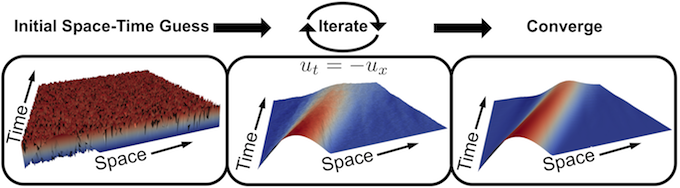
\includegraphics[width=1.0\textwidth]{Schematics/XBraid}
\caption{Multigrid in time with XBraid by LLNL\cite{XBraid}}
\label{fig:xbraid}
\end{figure}

Multigrid in time allows all times to be solved for simultaneously, dramatically improving parallelization opportunities within a
simulation code, see Figure~\ref{fig:xbraid}.
The practical downside is that this is a much more expensive procedure on small to medium sized computer architectures.
It's only on very large systems that have maxed out the strong scaling of a single timestep where this approach starts to pay off.
Thus, for the proof of concept problems solved on moderate sized system in this dissertation, we only expect to reap the extra cost
without seeing the reward.
However this concept has potential as we look towards exascale simulations in the future.

\subsection{Discontinuous Petrov-Galerkin Method}
The discontinuous Petrov-Galerkin finite element method with optimal test functions
% was first proposed by Demkowicz and Gopalakrishnan in 2009\cite{DPG1,DPG2}.
was first proposed by Demkowicz and Gopalakrishnan in 2009\cite{DPG2}.
The basic ideas are fairly straight-forward; DPG minimizes the residual in a user defined energy norm.
Consider a variational problem: find $u\in U$ such that
\[
b(u,v)=l(v) \quad\forall v\in V
\]
with operator $B:U\rightarrow V'\quad$ ($V'$ is the dual space to $V$) defined by $b(u,v)=\LRa{Bu,v}_{V'\times V}$.
This gives the operator equation:
\[
Bu=l\in V'\,.
\]
We wish to minimize the residual $Bu-l$ in $V'$:
\[
u_h=\argmin_{w_h\in U_h}\frac{1}{2}\norm{Bu-l}^2_{V'}\,.
\]
This is a very natural mathematical framework based soundly in functional analysis, but it is not yet a practical method as the $V'$ norm is not
especially tractable to work with.
The insight is that since we are working with Hilbert spaces, we can use the Riesz representation theorem to find a complementary object
in $V$ rather than $V'$. Let $R_V:V\ni v\rightarrow(v,\cdot)\in V'$ be the Riesz map.
Then the inverse Riesz map (which is an isometry) lets us represent our residual in $V$:
\[
u_h=\argmin_{w_h\in U_h}\frac{1}{2}\norm{R_V^{-1}(Bu-l)}^2_{V}\,.
\]
Taking the G\^ateaux derivative to be zero in all directions $\delta u \in
U_h$ gives,
\[
\left(R_V^{-1}(Bu_h-l),R_V^{-1}B\delta u\right)_V = 0, \quad \forall \delta u \in U,
\]
which by definition of the Riesz map is equivalent to
\begin{equation*}
\LRa{Bu_h-l,R_V^{-1}B\delta u_h}=0\quad\forall\delta u_h\in U_h\,,
\end{equation*}
with optimal test functions $v_{\delta u_h}\coloneqq R_V^{-1}B\delta u_h$ for each trial function $\delta u_h$.
This gives a simple bilinear form
\begin{equation*}
b(u_h,v_{\delta u_h})=l(v_{\delta u_h}),
\end{equation*}
with $v_{\delta u_h}\in V$ that solves the auxiliary problem
\begin{equation*}
\LRp{v_{\delta u_h},\delta v}_V=\LRa{R_Vv_{\delta u_h},\delta v}
=\LRa{B\delta u_h,\delta v}=b(\delta u_h,\delta v)\quad\forall\delta v\in V.
\end{equation*}
We might call this an \emph{optimal Petrov-Galerkin}.
We arrive at the same method by realizing the supremum in the inf-sup condition, motivating the \emph{optimal} nomenclature.
These optimal Petrov-Galerkin methods produce Hermitian, positive-definite stiffness matrices since
\[
b(u_h,\vdeltau)=(v_{u_h},\vdeltau)_V=\overline{(\vdeltau,v_{u_h})}=\overline{b(\delta u_h,v_{u_h})}\,.
\]
We can calculate the energy norm (defined by $\norm{u}_E:=\norm{Bu}_{V'}$) of the Galerkin error without knowing the exact solution by using the residual:
\[
\norm{u_h-u}_E=\norm{B(u_h-u)}_{V'}=\norm{Bu_h-l}_{V'}=\norm{R_V^{-1}(Bu_h-l)}_V\,,
\]
where we designate $R_V^{-1}(Bu_h-l)$ the \emph{error representation function}.
This has proven to be a very reliable \emph{a-posteriori} error estimator for driving adaptivity.

Babu\v{s}ka's theorem\cite{Babuska70} says that discrete stability and approximability imply convergence.
That is, if $M$ is the continuity constant for $b(u,v)$ which satisfies the discrete inf-sup condition with constant $\gamma_h$,
\[
\sup_{v_h\in V_h}\frac{|b(u,v)|}{\norm{v_h}_V}\geq\gamma_h\norm{u_h}_U\,,
\]
then the Galerkin error satisfies the bound
\[
\norm{u_h-u}_U\leq\frac{M}{\gamma_h}\inf_{w_h\in U_h}\norm{w_h-u}_U\,.
\]
Optimal test functions realize the supremum in the discrete discrete inf-sup condition such that $\gamma_h\geq\gamma$,
the infinite-dimensional inf-sup constant.
If we then use the energy norm for $\norm{\cdot}_U$, then $M=\gamma=1$ and Babu\v{s}ka's estimate implies that
the optimal Petrov-Galerkin method is the most stable Petrov-Galerkin method possible.

There are still many features of the method that are left to be decided, for example the $U$ and $V$ spaces.
If $V$ is taken to be a continuous space, then the auxiliary problem becomes global in scope, something that we would like to avoid.
In order to ensure the auxiliary problem can be solved element-by-element, we take $V$ to be discontinuous between elements.
(Technically, $V$ should also be infinite dimensional, but we have found it to be sufficient to use an ``enriched'' space of higher
polynomial dimension than the trial space.)
The downside to using discontinuous test functions is that it introduces new interface unknowns.
When the equations are integrated by parts over each element, the jump in test functions introduces new unknowns on the mesh skeleton
that would have gone away with continuous test functions.
Moro \etal\cite{MoroNguyenPeraire11} handle the flux unknowns with a numerical flux in the hybridized DPG method, but the standard DPG method treats
these as new unknowns to be solved for.
We still haven't specified our trial space $U$, but the rule is that for every integration by parts, a new skeleton unknown is introduced.
Most DPG considerations break a second order PDE into a system of first order PDEs which introduces a trace unknown (from the constitutive law)
and a flux unknown (from the conservation law), but Demkowicz and Gopalakrishnan also formulated a \emph{primal DPG} method for second order equations
that does not introduce a trace unknown.
The overall number of interface unknowns in the primal DPG method is the same, however, since the solution is required to be $H^1$ conforming
and the trace unknowns are essentially hidden here.

The final unresolved choice is what norm to apply to the $V$ space.
This is one of the most important factors in designing a robust DPG method as this norm needs to be inverted to solve for the optimal test functions.
If the norm produces unresolved boundary layers in the auxiliary problem, then many of the attractive features of DPG may fall apart.
But elimination of boundary layers in the auxiliary solve is not the only requirement at play.
This choice also controls what norm the residual is minimized in.
Often we want this norm to be equivalent to the $L^2$ norm.
Fortunately, we have found that it is possible to design test norms such that the implied energy norm
is provably robust and equivalent to $L^2$ for convection-diffusion which
serves as the most relevant model problem for our research.
Norms for Navier-Stokes are derived by analogy to the convection-diffusion norm.

DPG has been successfully applied to a wide range of physical problems.
Early work on the Poisson equation was published in \cite{DPGPoisson}.
Demkowicz \etal\cite{DPGHelmholtz}, Gopalakrishnan \etal\cite{Gopalakrishnan2014}, and Zitelli \etal\cite{DPG4}
analyzed and solved the Helmholtz equation with DPG.
DPG was applied to linear elasticity and plate problems in \cite{BramwellDPG}, \cite{NiemiBramwellDemkowicz10}, and \cite{BramwellDemkowiczQiu10}.
A 2D Maxwell cloaking problem was solved with DPG in \cite{DPGCloaking}
and a 3D DPG theory for Maxwell was developed by Wieners and Wohlmuth\cite{WohlmuthReport}.
DPG has been applied to various fluid problems including convection-diffusion\cite{DPG3,DemkowiczHeuer,ChanHeuerThanhDemkowicz2012,Chan2013,EllisLC},
Stokes\cite{DPGStokes,EllisLC}, Burgers' equation\cite{Chan2013dpg}, incompressible Navier-Stokes\cite{NateDissertation,RobertsDPGNavierStokes},
and compressible Navier-Stokes\cite{JesseDissertation}.

\paragraph{Camellia -- A Library for Computing with DPG.}
DPG is a relatively young technology and has some fairly unique implementation requirements. 
In particular, the use of element interface unknowns, the computation of the optimal test functions,
and the use of the error representation function to drive adaptivity are not common
features in many finite element libraries.
Nathan Roberts began work on the Camellia\cite{CamelliaDPG} library the summer of 2011 at Sandia National Laboratory.
% Jesse Chan and I quickly became active contributors when we saw the promising early demonstrations.
Jesse Chan and I soon followed as active contributors.
Camellia is written in modern C++ on top of Trilinos\cite{Trilinos} and supports distributed computation with MPI.
It currently supports 1D, 2D, and 3D meshes with line, quadrilateral, triangle,
hexahedral, and tetrahedral elements as well as space-time in 1D and 2D and both $h-$ and $p-$adaptivity.
Though Camellia has not undergone an official open source release yet and many of the features are still experimental,
the source code is available at \cite{CamelliaGitHub}.
Every numerical result in this dissertation was computed using Camellia.

% \section{Goal}
% The goal of this work is to develop a space-time formulation of DPG with the purpose of simulating transient
% fluid dynamics problems.
% The emphasis will be on incompressible Navier-Stokes, but we also intend to study the compressible equations.
% We will also consider the convection-diffusion equation as a simplified model for developing robust space-time DPG methods.

% \subsection{Organization of this Proposal}
% This proposal is organized as follows.
% In Chapter~\ref{sec:conservation}, I summarize my past work developing a locally conservative DPG formulation for steady-state problems.
% I develop the method by augmenting the DPG system with Lagrange multipliers, then prove stability and robustness of the new formulation.
% Several numerical experiments are shown for convection-diffusion, Burgers' equation, and Stokes flow that demonstrate the effectiveness of the method.
% There is no reason the locally conservative formulation would not work in space-time; in fact I've done some preliminary simulations
% (not covered in this proposal) for 1D compressible Navier-Stokes that seem to confirm that everything works as expected.
% Of course, for problems as simple as 1D shock tubes, local conservation doesn't affect the solutions very much.
%
% Chapter~\ref{sec:timestepping} covers some exploratory work on coupling DPG with time stepping techniques.
% In particular, I single out the explicit singly diagonal implicit Runge-Kutta (ESDIRK) methods as promising options for
% coupling with DPG.
% Ultimately, we decided that space-time DPG offered a more attractive option, but time stepping techniques are not disqualified as a possibility.
%
% Chapter~\ref{sec:spacetime} presents the completed work so far on developing space-time DPG for 1D problems.
% The heat equation serves as a useful model as it is the simplest parabolic (first order in time, second order in space) problem.
% The ideas developed for the heat equation translate directly to convection-diffusion and the transient compressible Navier-Stokes equations.
% I present some preliminary results for several 1D shock tube problems.
%
% Finally, Chapter~\ref{sec:proposed} presents my proposed plans for this dissertation, emphasizing 2D space-time problems and development of
% a mathematical theory for space-time DPG.
% I then summarize my contributions to areas A, B, and C according to the ICES Ph.D. requirements.

\end{document}
